\documentclass[12pt,aspectratio=169]{beamer}
\usetheme{default}
\usecolortheme{dolphin}
\usefonttheme{structurebold}
\setbeamertemplate{footline}[frame number]

\title{ShellScript 01}
\author{@aoirint}
\date{2020/04/16}
%\institute{}

\begin{document}

% 01
\frame{\maketitle}

% 02
\begin{frame}{テキスト}

  \begin{minipage}{0.58\textwidth}
    \begin{itemize}
      \item 新しいシェルプログラミングの教科書
      \begin{itemize}
        \item 著・三宅英明
        \item 刊・SB Creative
      \end{itemize}
    \end{itemize}
  \end{minipage}
  \hfill
  \begin{minipage}{0.38\textwidth}
    \vspace{-4\baselineskip}
    \begin{center}
      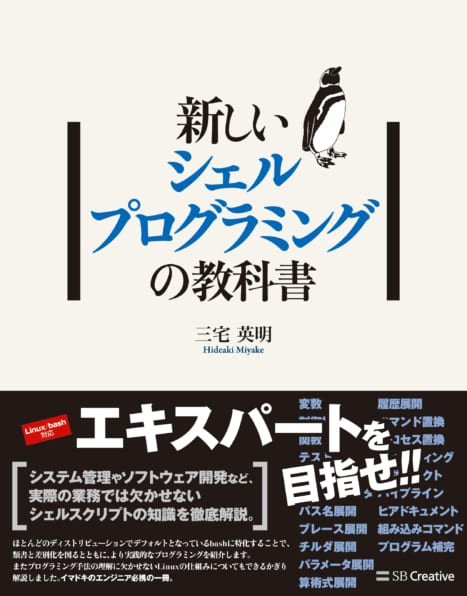
\includegraphics[width=5cm,bb=0 0 467 596]{./images/shellbook.jpg}
    \end{center}
  \end{minipage}

  \begin{itemize}
    \item 書影
    \begin{itemize}
      \item { \small \url{https://www.sbcr.jp/product/4797393101/} }
    \end{itemize}
  \end{itemize}

\end{frame}


\begin{frame}{シェル:GUI(Graphical User Interface)}

  \begin{minipage}{0.45\textwidth}
    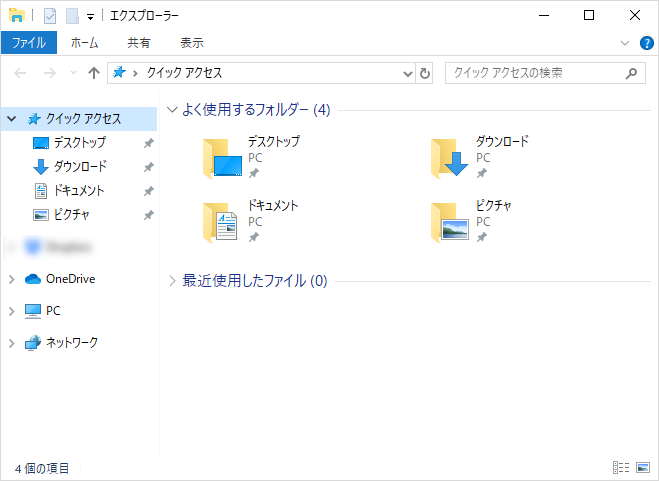
\includegraphics[width=6cm,bb=0 0 659 481]{./images/explorer.png}
    Explorer(Windows)
  \end{minipage}
  \hfill
  \begin{minipage}{0.45\textwidth}
    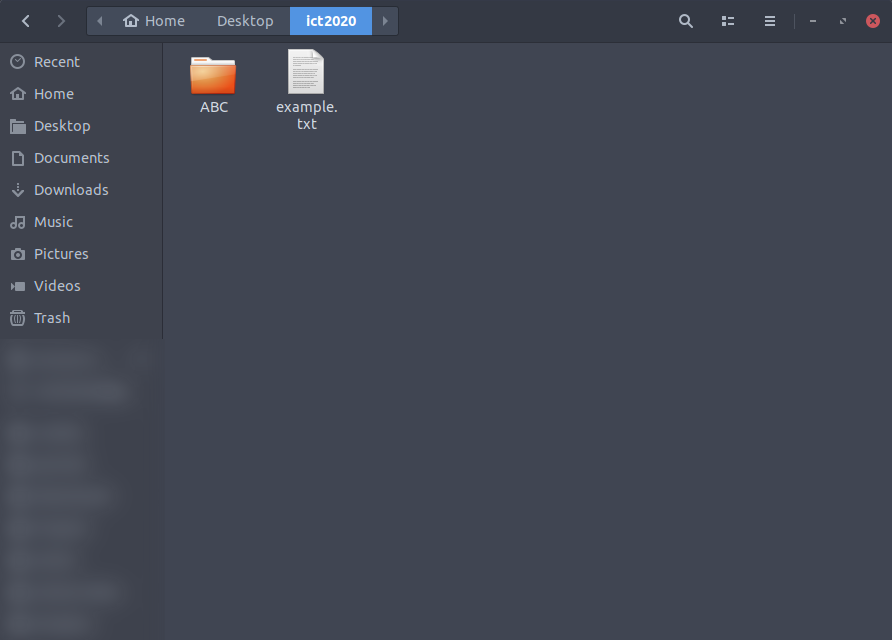
\includegraphics[width=6cm,bb=0 0 892 640]{./images/nautilus.png}
    Nautilus(Ubuntu, Gnome)
  \end{minipage}

\end{frame}


\begin{frame}{シェル:CLI(Command Line Interface)}

  \begin{minipage}{0.3\textwidth}
    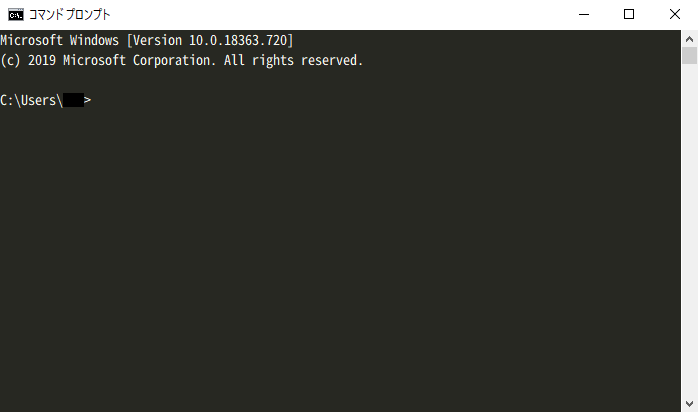
\includegraphics[width=1.2\linewidth,bb=0 0 698 412]{./images/cmd.png}
    コマンドプロンプト(Windows)

    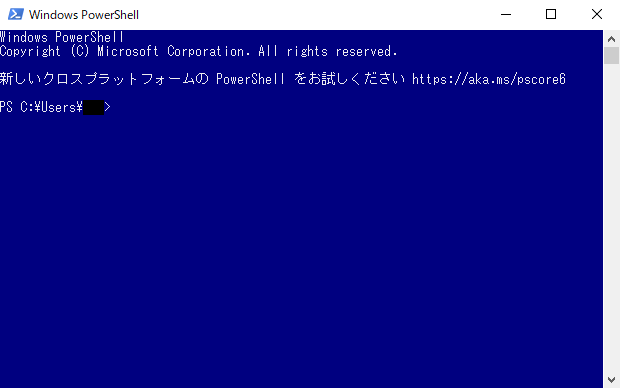
\includegraphics[width=1.2\linewidth,bb=0 0 620 388]{./images/powershell.png}
    PowerShell(Windows)
  \end{minipage}
  \hfill
  \begin{minipage}{0.3\textwidth}
    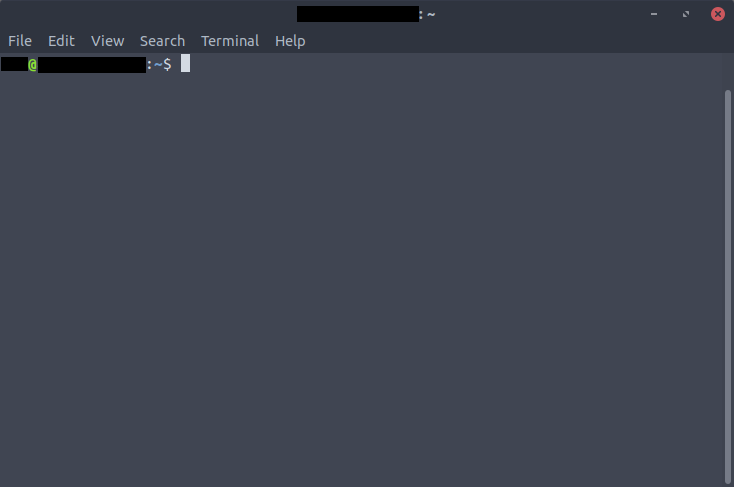
\includegraphics[width=\linewidth,bb=0 0 734 487]{./images/ubuntu-gnome.png}
    \begin{flushleft} \small Terminal(Ubuntu,Gnome) \end{flushleft}
    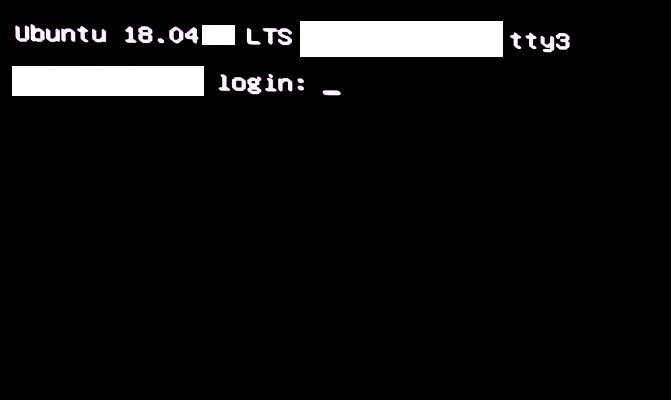
\includegraphics[width=\linewidth,bb=0 0 734 487]{./images/ubuntu-cli.jpg}
    CLI(Ubuntu)
  \end{minipage}
  \hfill
  \begin{minipage}{0.3\textwidth}
    \vspace{-5\baselineskip}
    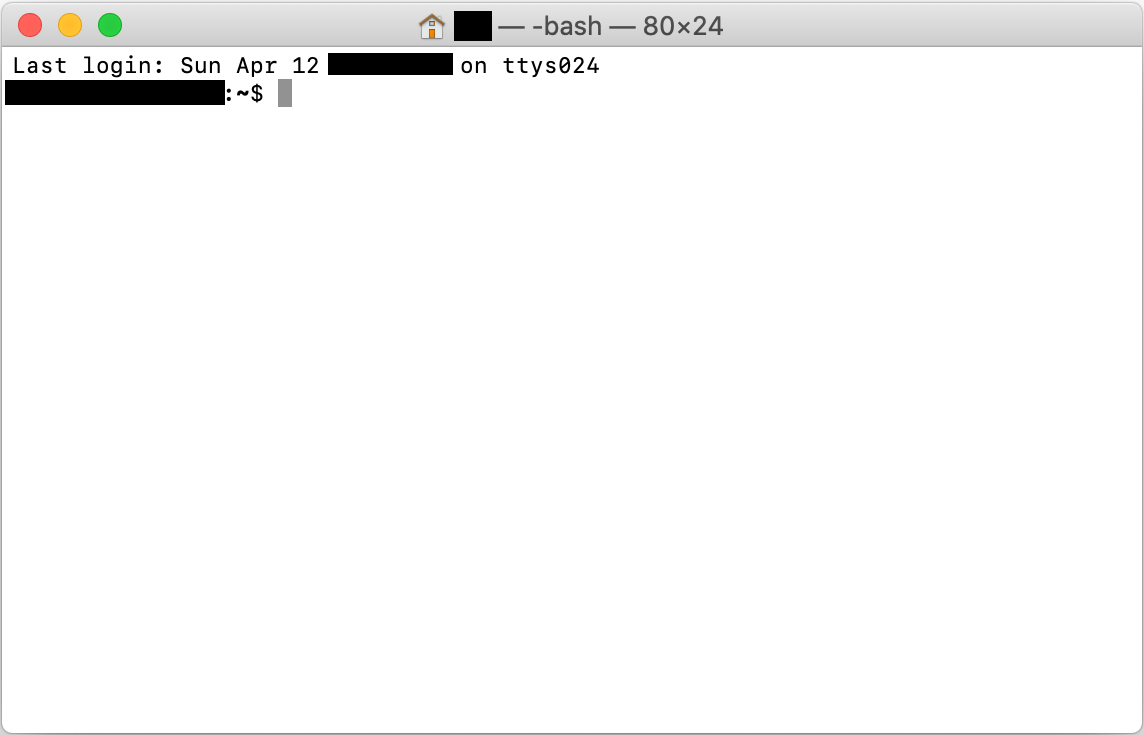
\includegraphics[width=2.0\linewidth,bb=0 0 1144 735]{./images/mac-basic.png}
    Terminal(macOS)
  \end{minipage}

\end{frame}

\begin{frame}{シェルはどこに位置するか}
  \centering
  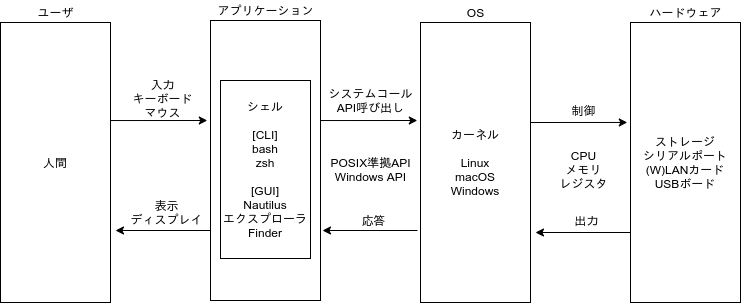
\includegraphics[width=12cm,bb=0 0 741 281]{./images/shell.png}

\end{frame}

\begin{frame}{OSとカーネル}
  \begin{itemize}
    \item カーネル(Kernel)
      \begin{itemize}
        \item OSの核となる(中心的な)機能の実装
          \begin{itemize}
            \item ファイルシステム、ネットワーク、入出力、プロセス管理など
          \end{itemize}
        \item 例:Linuxカーネル、macOSカーネル(XNU)、Windowsカーネル
        \item 余談:Linuxディストリビューションと呼ばれるOSのカーネルはLinuxカーネルをベースにしている
          \begin{itemize}
            \item Debian GNU/Linux、Ubuntu、CentOSなど
          \end{itemize}
      \end{itemize}

      \item OS
        \begin{itemize}
          \item カーネルにハードウェアドライバや標準のソフトウェアなどを追加したパッケージ
          \item 例:Ubuntu、CentOS、macOS、Windows(バージョン略)
        \end{itemize}

      \item 例:C言語のfopen, fprintf, fcloseはファイルシステムに関するカーネルの機能を(最終的に)呼び出す関数(システムコール)
  \end{itemize}

\end{frame}


\begin{frame}{シェルとコマンド 1/2}
  \begin{itemize}
    \item シェル(Shell)
      \begin{itemize}
        \item コマンドによりカーネルの機能を利用するためのアプリケーションの一種
          \begin{itemize}
            \item 例:ファイルの作成、削除、プロセス管理、他のアプリケーションの起動
          \end{itemize}
        \item ユーザに提供されるコマンドベースのカーネルへのインタフェース
          \begin{itemize}
            \item カーネル/核 の 殻/シェル
          \end{itemize}
        \item 例:sh, bash, zsh, csh, コマンドプロンプト(cmd.exe), PowerShellなど
        \item *shという名前のシェルはよく共通のコマンドを持っている
      \end{itemize}
    \item シェルのコマンド
      \begin{itemize}
        \item 例:*shのコマンドls、cmd.exeのコマンドdir、PowerShellのコマンドGet-ChildItemはディレクトリ中のファイルリストを表示する
      \end{itemize}
  \end{itemize}

\end{frame}


\begin{frame}{シェルとコマンド 2/2}
  \begin{itemize}
    \item シェルのコマンド
      \begin{itemize}
        \item 例:*shのコマンドls、cmd.exeのコマンドdir、PowerShellのコマンドGet-ChildItemはディレクトリ中のファイルリストを表示する
      \end{itemize}
  \end{itemize}

  \centering {
    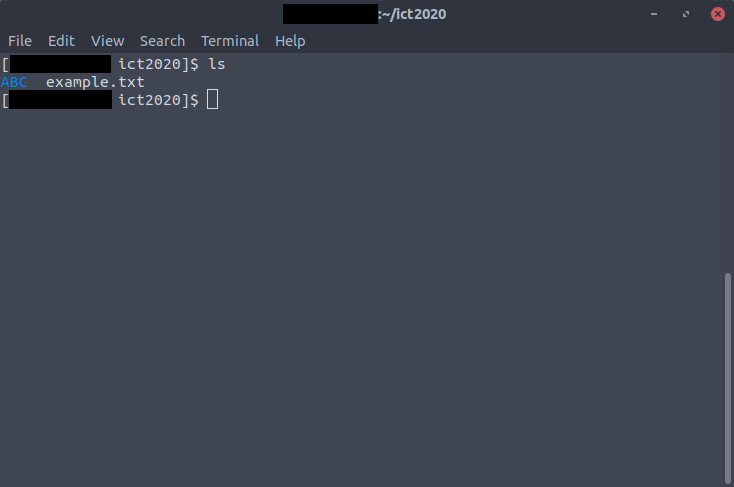
\includegraphics[width=6cm,bb=0 0 659 481]{./images/ls.png}
  }

\end{frame}


\begin{frame}{Explorerもシェル}

  \begin{minipage}{0.45\textwidth}
    \begin{itemize}
      \item Explorer(Windows)もシェル
        \begin{itemize}
          \item GUIなのにコマンド?
        \end{itemize}
      \item 例:コンテキストメニュー(右クリックメニュー)の動作
        \begin{itemize}
          \item レジストリ中にテキスト形式のコマンドで定義されている
          \item { \tiny 余談 }
            \begin{itemize}
              \item { \tiny レジストリを編集すれば自分でメニューを追加することもできる(間違ったところをいじらないように注意は必要) }
              \item { \tiny u\_atomhere, u\_conemuhereは自分で追加した項目 }
            \end{itemize}
        \end{itemize}
    \end{itemize}

  \end{minipage}
  \hfill
  \begin{minipage}{0.45\textwidth}
    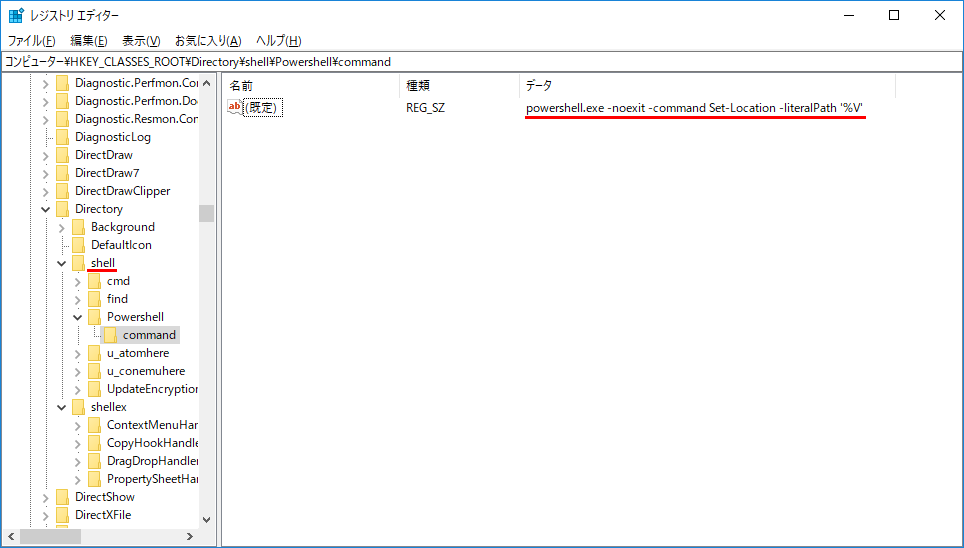
\includegraphics[width=6cm,bb=0 0 659 481]{./images/regedit.png}
    { \tiny Windowsのレジストリ(フォルダをShift+右クリックしたときの「PowerShellで開く」コマンド) }
  \end{minipage}

\end{frame}


\begin{frame}{ログインシェル}
  \begin{itemize}
    \item テキストではbashを題材にしているので、ここからはbashを前提とする
      \begin{itemize}
        \item なお、デフォルトのシェルをログインシェルという
        \item ログインシェルの指定はユーザ情報を保管するファイル/etc/passwdなどに書かれている
      \end{itemize}

  \end{itemize}

\end{frame}
\begin{frame}{シェルとプロセス 1/2}
  \begin{itemize}
    \item プロセスの親子関係
      \begin{itemize}
        \item シェル上でコマンドを実行したとき、シェルのプロセスに対する子プロセスが生成される
      \end{itemize}
    \item 子プロセス
      \begin{itemize}
        \item 親となるプロセスのメモリ内容(アドレス空間)をコピーして作られる
        \item メモリがコピーされているため、親プロセスのシェル上の環境変数などを引き継ぐ
        \item プログラムを呼び出すコマンドが実行されると、forkシステムコールにより子プロセスが生成されたあと、exec系システムコールによりプログラムが子プロセスのアドレス空間(メモリ領域)に読み出される
      \end{itemize}

  \end{itemize}

\end{frame}


\begin{frame}{シェルとプロセス 2/2}
  \begin{itemize}
    \item psコマンド
      \begin{itemize}
        \item プロセスリストを表示するコマンド
        \item ps fはプロセスの親子関係をグラフィカルに表示する
      \end{itemize}
  \end{itemize}

  \centering {
    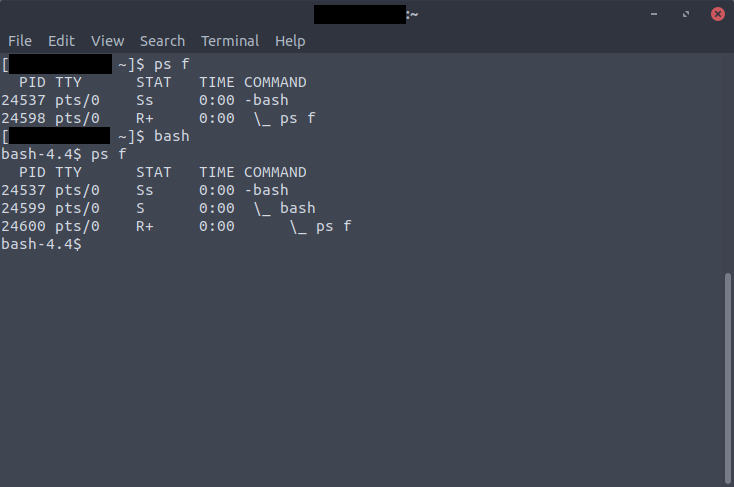
\includegraphics[width=6cm,bb=0 0 734 487]{./images/child-process.png}
  }

  \begin{itemize}
    \item 親プロセスはbash(ID 24537)、プログラム/usr/bin/bashを呼び出して子プロセスbash(ID 24599)が生成されている
      \begin{itemize}
        \item また、psコマンド自体も子プロセスとして実行されている
      \end{itemize}
  \end{itemize}

\end{frame}


\begin{frame}{シェルスクリプトとは}
  \begin{itemize}
    \item シェルのコマンドを列挙したテキストファイル
    \item ファイルをシェルプログラムに与えることで実行する
    \item 複数のコマンドや複雑なコマンドをいちいち入力する必要がなくなる
      \begin{itemize}
        \item 複数のコマンド
          \begin{itemize}
            \item コマンドを組み合わせた定型処理
          \end{itemize}
        \item 複雑なコマンド
          \begin{itemize}
            \item たくさんのオプションを指定するプログラム
            \item 例:動画像・音声処理プログラムのffmpegなど
          \end{itemize}
        \item if, forなどの制御構造を含むプログラム
        \item 起動時・ログイン時の初期化プログラム
      \end{itemize}
  \end{itemize}

\end{frame}


\begin{frame}{シェルスクリプトを実行する}
  \begin{itemize}
    \item command.shファイルを作成(echoは文字列を出力するコマンド) \\
      \texttt {
        echo "Hello Shell Script!"
      }
    \item \texttt{bash command.sh} で実行
  \end{itemize}

  \centering {
    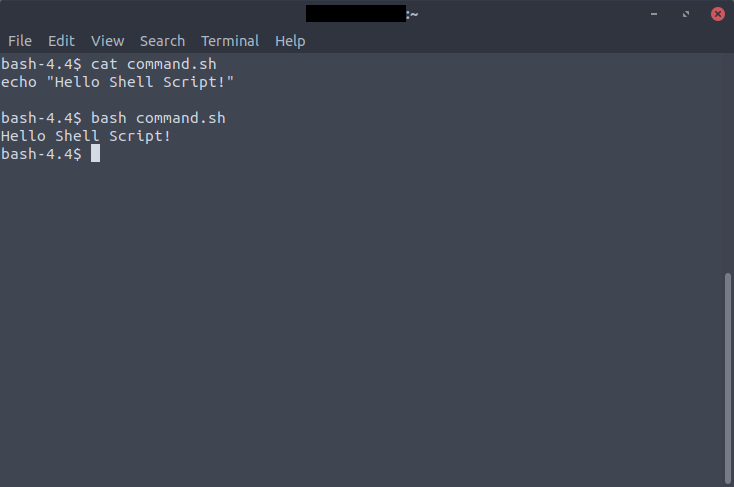
\includegraphics[width=6cm,bb=0 0 734 487]{./images/exec-sh.png}
  }

\end{frame}


\begin{frame}{shebang}
  \begin{itemize}
    \item command.shの1行目に以下を追記する \\
      \texttt {
        !\#/bin/bash
      }
      \begin{itemize}
        \item これはshebangという記法(/bin は /usr/bin へのシンボリックリンク)
        \item ファイルの実行時にファイルパスを渡すプログラムを記述する(シェルでなくてもよい; ex.CGIスクリプト)
      \end{itemize}
    \item command.shに実行権限を付与する \\
      \texttt {
        chmod +x command.sh
      }
    \item \texttt{./command.sh} で実行
      \begin{itemize}
        \item \texttt{command.sh}を\texttt{command}にリネームすると\texttt{./command}で実行できる
      \end{itemize}

  \end{itemize}

  \centering {
    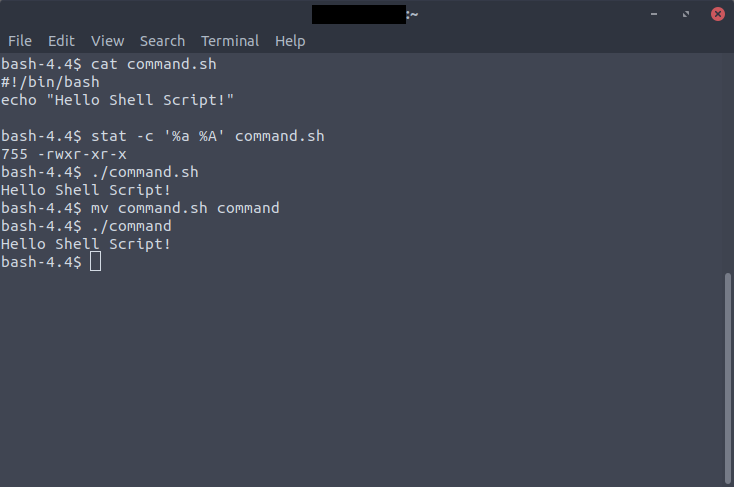
\includegraphics[width=6cm,bb=0 0 734 487]{./images/exec-sh2.png}
  }

\end{frame}


\begin{frame}{シェルスクリプトの記法}
  \begin{itemize}
    \item 改行
      \begin{itemize}
        \item コマンドとコマンドの区切りは改行で表される
        \item コマンドの途中で改行するときはバックスラッシュ( $\backslash$ )を入れる
          \begin{itemize}
            \item 改行は空白扱いにはならないので注意
            \item ×:\texttt{echo$\backslash$[改行]Hello}
            \item ◯:\texttt{echo $\backslash$[改行]Hello}
            \item ◯:\texttt{ec$\backslash$[改行]ho Hello}
          \end{itemize}

        \item 空行(何も書かれていない行)は無視される
      \end{itemize}

    \item コメント
      \begin{itemize}
        \item 実行されないテキストをスクリプト中に埋め込める
        \item 文字\#以降のその行はコメント\\
          \texttt{echo Hello \# shell say Hello }
        \item コメントアウト(コマンドをコメントにして実行されないようにする)\\
          \texttt{\# echo Hello }
      \end{itemize}

  \end{itemize}

\end{frame}

\begin{frame}{カレントディレクトリ}
  \begin{itemize}
    \item pwd(positioning working directory)コマンド\\
      \texttt{pwd}
      \begin{itemize}
        \item カレントディレクトリを出力する(echoのように)
        \item 相対パスの基点となる
          \begin{itemize}
            \item 絶対パスの例:/home/user/command.sh
            \item 相対パスの例:command.sh または ./command.sh, ../example.txt (.はカレントディレクトリ、..は親ディレクトリを意味する)
          \end{itemize}
      \end{itemize}

    \item cd(change directory)コマンド\\
      \texttt{cd MY\_PATH}
      \begin{itemize}
        \item カレントディレクトリを\texttt{MY\_PATH}に変更する
      \end{itemize}

    \item カレントディレクトリ以外のファイルも実行できる/扱える
      \begin{itemize}
        \item カレントディレクトリが異なると 相対パスで指定したファイルを操作するときの操作対象が変わる
      \end{itemize}

  \end{itemize}

\end{frame}


\begin{frame}{以上です}
てすと

\end{frame}


\begin{frame}{参考資料:Beamer}
  \begin{itemize}
    \item \url { https://qiita.com/yt_siden/items/aaac54f6389a8068a4ee }
    \item \url { https://qiita.com/termoshtt/items/756aec542fb4c812a405 }
    \item \url { https://www.opt.mist.i.u-tokyo.ac.jp/~tasuku/beamer.html }
  \end{itemize}

\end{frame}


\begin{frame}{参考資料:OS, カーネル}
  \begin{itemize}
    \item \url { https://ja.wikipedia.org/wiki/Microsoft_Windows }
    \item \texttt {https://ja.wikipedia.org/wiki/Linux\%E3\%83\%87\%E3\%82\%A3 \\ \%E3\%82\%B9\%E3\%83\%88\%E3\%83\%AA\%E3\%83\%93\%E3\%83\%A5\%E3\%83\%BC \\ \%E3\%82\%B7\%E3\%83\%A7\%E3\%83\%B3 }
    \item \url { https://ja.wikipedia.org/wiki/POSIX }
    \item \url { https://ja.wikipedia.org/wiki/Debian }
    \item \url { https://ja.wikipedia.org/wiki/MacOS }
    \item \url { https://ja.wikipedia.org/wiki/XNU }
    \item \url { https://www.atmarkit.co.jp/ait/articles/1112/13/news117.html }
    \item \texttt {https://ja.wikipedia.org/wiki/\%E3\%82\%AA\%E3\%83\%9A \\ \%E3\%83\%AC\%E3\%83\%BC\%E3\%83\%86\%E3\%82\%A3\%E3\%83\%B3\%E3\%82\%B0 \\ \%E3\%82\%B7\%E3\%82\%B9\%E3\%83\%86\%E3\%83\%A0 }
  \end{itemize}

\end{frame}

\begin{frame}{参考資料:プロセス}
  \begin{itemize}
    \item \url { https://ja.wikipedia.org/wiki/Fork }
    \item \url { https://kazmax.zpp.jp/linux_beginner/process_ps.html }
  \end{itemize}

\end{frame}


\begin{frame}{参考資料:スクリプト}
  \begin{itemize}
    \item https://docs.microsoft.com/ja-jp/powershell/scripting/samples/\\ working-with-files-and-folders
    \item \url { https://ja.wikipedia.org/wiki/Pwd }
  \end{itemize}

\end{frame}


\end{document}
